\chapter{Pruebas de carga en sistema} \label{ch:carga_cliente}

En este capítulo profundizaremos sobre la monitorización de un sistema, en este caso supondrá un sistema en \textbf{WordPress}, este se trata de un sistema de gestión de contenidos.

A través de la herramienta \textbf{Naemon} y el framework de \textbf{Locust} queremos realizar el análisis de dicho sistema.
\section{Despliegue de sistema a través del contenedor Docker}
Como se realizó en capítulos anteriores para realizar el despliegue de Naemon y Locust en Docker, esta vez pasaremos a la realización del despliegue de WordPress. Para ello nos basaremos en dos instancias separadas: \textbf{una instancia para Wordpress} y \textbf{otra instancia separada para MySQL con un volumen montado para la persistencia de los datos de MySql}.

En él definimos dos \textbf{servicios}: \textbf{db} (correspondiente a MySQL) y \textbf{wordpress}. En el \textbf{primer servicio (db)} indicamos la imagen que queremos descargarnos (un MySQL versión 5.7) y algunos parámetros de configuración. Los más relevantes son la redirección de puertos (del 8081 del anfitrión al 3306 del huésped) y parámetros de la base de datos en sí (usuario, contraseña, etc).
\newpage
El \textbf{segundo servicio es WordPress (wordpress)} y sigue un patrón parecido. Aquí, por ejemplo, indicamos que queremos usar el puerto 80 para acceder a nuestro WordPress. También especificamos que db es una dependencia de WordPress (este contenedor no puede funcionar sin el otro) esto lo haremos mediante la opción \textbf{depends on}. Y también indicamos parámetros adicionales como, por ejemplo, dónde está la base de datos y cómo acceder a ella. Todo esto vendrá definido en el archivo \textbf{docker-compose.yml} de la siguiente manera:
\begin{lstlisting}[language=bash]
db:
	image: mysql:5.7
	volumes:
	 - db_data:/var/lib/mysql
	restart: always
	environment:
		MYSQL_ROOT_PASSWORD: somewordpress
		MYSQL_DATABASE: wordpress
		MYSQL_USER: wordpress
		MYSQL_PASSWORD: wordpress

wordpress:
	depends_on:
	 - db
	image: wordpress:latest
	ports:
	 - "80:80"
	restart: always
	environment:
		WORDPRESS_DB_HOST: db:3306
		WORDPRESS_DB_USER: wordpress
		WORDPRESS_DB_PASSWORD: wordpress
		WORDPRESS_DB_NAME: wordpress
\end{lstlisting}
Si realizamos la puesta en marcha mediante el comando \textbf{docker-compose up} comenzará con la descarga de las imágenes de \textbf{WordPress y MySQL}, y de forma seguida pondrá en funcionamiento el sistema de \textbf{WordPress}.

Cuando termine la instalación del contenedor, accedemos al navegador e introducimos la siguiente dirección \url{http://localhost:80} o \url{http://localhost}, donde se lanzará la instalación correspondiente de \textbf{WordPress}.
\newpage
\begin{figure}[H]
	\centering
	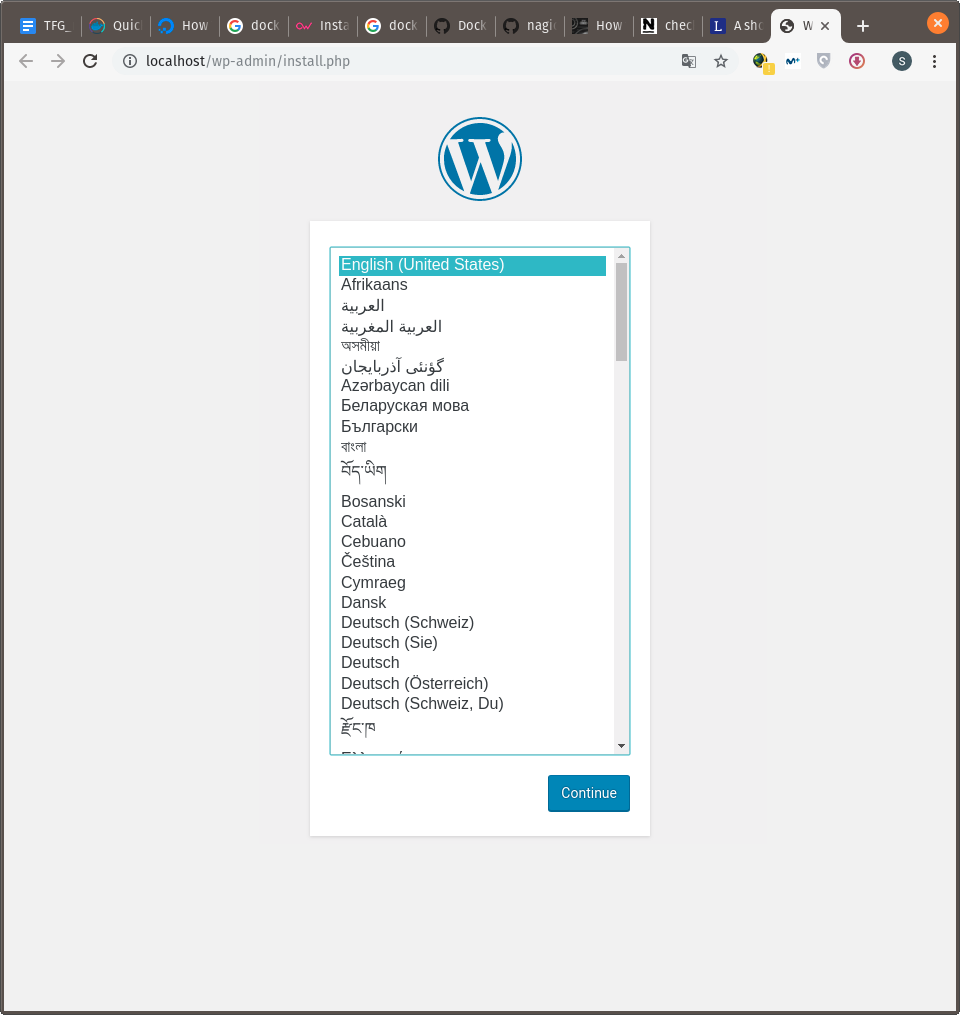
\includegraphics[scale=0.2]{imagenes/wordpress/wordpressinstall.png}
	\caption{Instalación de WordPress} \label{wordpress}
\end{figure}

Realizado este paso solo quedará instalar \textbf{WordPress} con el blog correspondiente que se quiera ejecutar, en este caso se ha llamado al blog \textbf{Monitorización TFG}:

\begin{figure}[H]
	\centering
	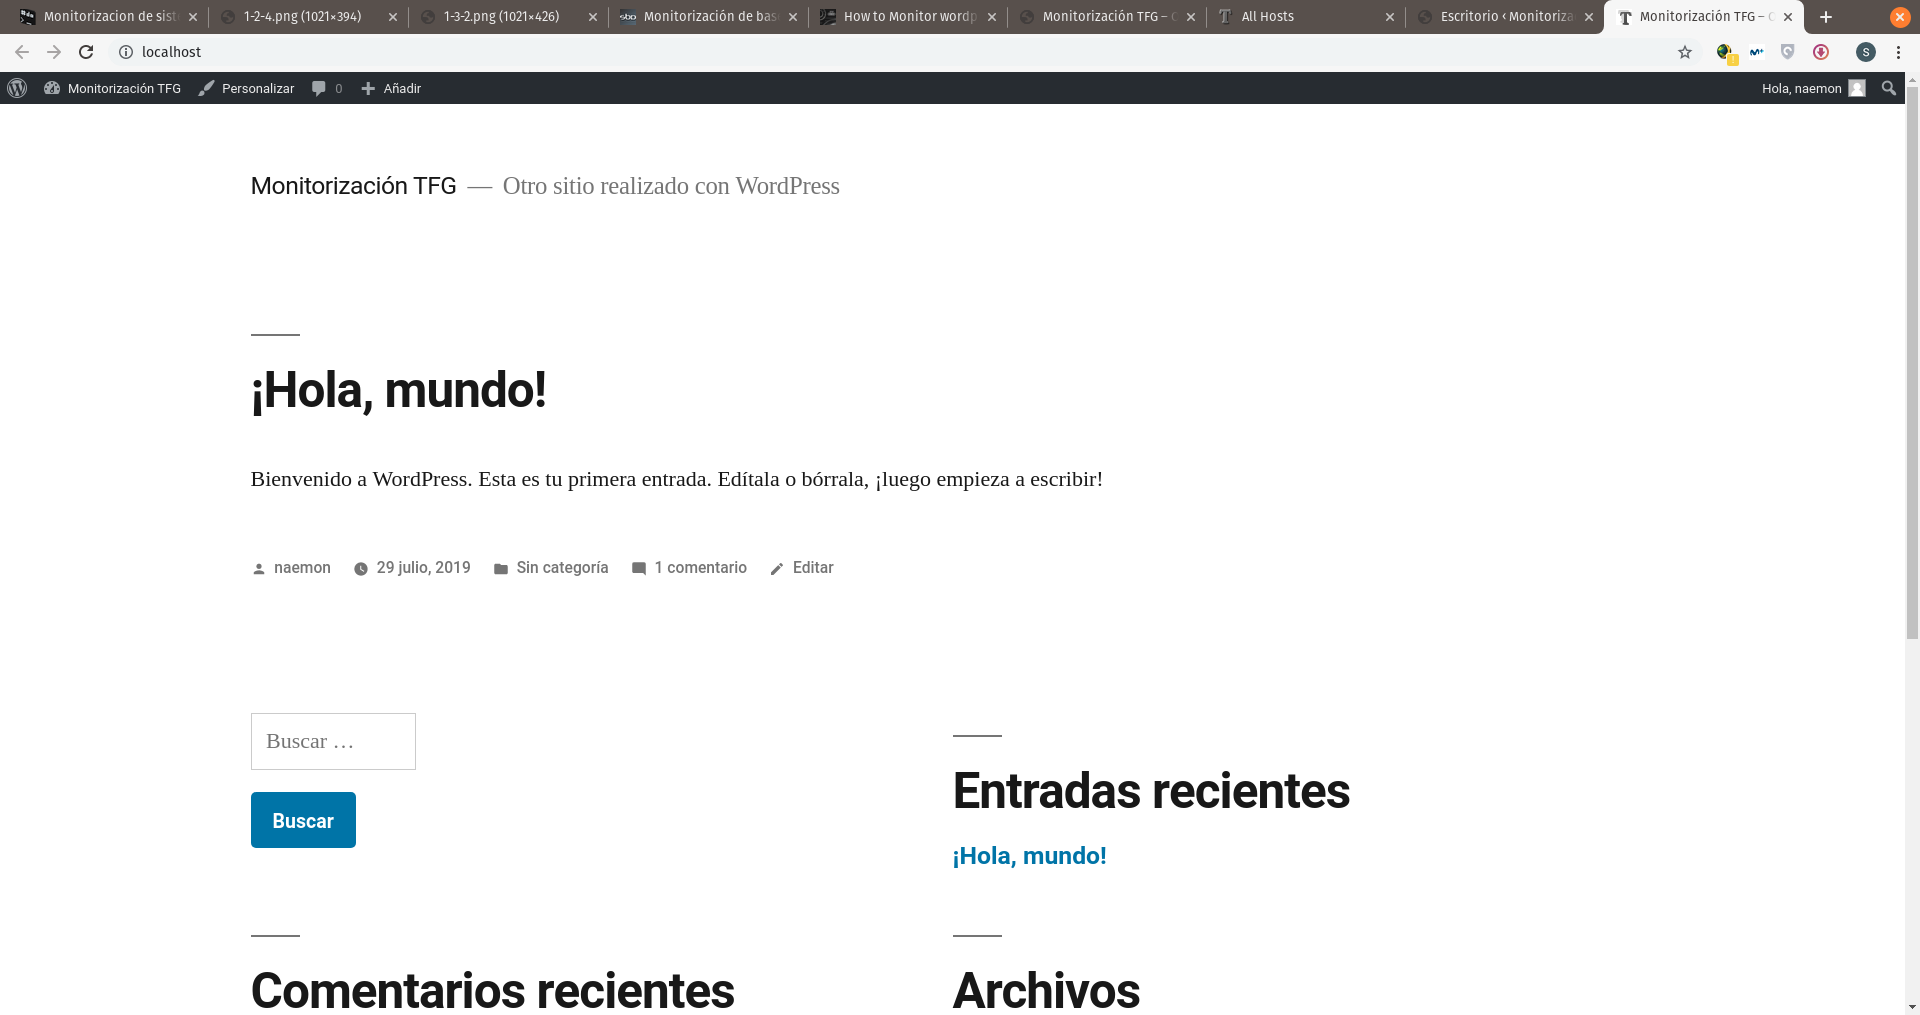
\includegraphics[scale=0.2]{imagenes/wordpress/instalacion-wordpress.png}
	\caption{Pantalla principal Blog de WordPress} \label{wordpress}
\end{figure}
\newpage
\section{Enlazado con Locust}
Como ya contamos con nuestro sistema montado sólo nos quedará realizar el enlazado con el \textbf{Framework de Locust}, para ello es necesario adaptar la configuración interna del archivo \textbf{locust.config.json}. Este archivo será añadido al fichero do\textbf{cker-compose.yml} junto al \textbf{locustfile.py}.

Dicho archivo nos servirá para especificar la \textbf{URL raíz de la API} a la que se va a redirigir la \textbf{API de Locust}, junto con la lista de nombres de clase para las subclases de Locust que se usarán en la prueba.

El archivo \textbf{JSON} que tendremos que crear será algo como el siguiente:

\begin{lstlisting}[language=json,firstnumber=1]
{
"target": "http://wordpress",
"locusts": ["WebsiteUser"]
}
\end{lstlisting}

Donde \textbf{target} corresponde a la dirección que vamos a capturar, especificamos  \url{http://wordpress} ya que wordpress coincide con la etiqueta de creación de la imagen de WordPress, se podría poner  \url{http://localhost} y funcionaría, pero esto garantiza que verdaderamente estamos estableciendo la relación con ese entorno, ya que a la hora de la realización se ha encontrado un problema con el paso de peticiones GET a través del servidor Apache y era necesario aplicar un cambio interno en la configuración de WordPress, estableciendo el puerto base como 80. Por lo que esta medida es garantizable y más rápida de realizar, ya que se está trabajando a través del despliegue de Docker.

La etiqueta \textbf{locusts} corresponde a la tarea o clase por la que vamos a ejecutar, en este caso es \textbf{WebsiteUser} que realiza toda la funcionalidad de nuestro archivo.
\newpage
\subsection{Creación de archivo Locustfile}

Como se realizó en capítulos anteriores para poder empezar a trabajar con \textbf{Locust} es necesario la creación del archivo \textbf{locustfile.py} para poder realizar las distintas pruebas de carga. Para ello analizaremos la prueba de carga a la hora de acceder y salir del sistema WordPress, además realizaremos una prueba de carga para un artículo concreto, esto se realizará mediante el lanzado de la petición \textbf{GET} hacia la URL \textbf{/?p=1}.

En el caso del \textbf{login} y el \textbf{logout}, lanzaremos peticiones \textbf{POST}, ya que éste tipo de petición se utiliza para enviar una entidad a un recurso en específico, causando a menudo un cambio en el estado o efectos secundarios en el servidor.

El código del archivo \textbf{locustfile.py} quedará de la siguiente manera:
\begin{lstlisting}[language=Python]
from locust import HttpLocust, TaskSet, task

def login(l):
l.client.post("/login", {"username":"naemon", "password":"naemon"})

def logout(l):
l.client.post("/logout", {"username":"naemon", "password":"naemon"})


class UserBehavior(TaskSet):
def on_start(self):
login(self)

def on_stop(self):
logout(self)
@task(2)
def root(self):
self.client.get('/')
@task(1)
def host(self):
self.client.get('/?p=1')
class WebsiteUser(HttpLocust):
task_set = UserBehavior
min_wait = 5000
max_wait = 9000


\end{lstlisting}

Si lanzamos en terminal el comando \textbf{docker-compose up} y lanzamos el enlace \url{http://localhost:8089/} ejecutaremos \textbf{Locust} a través del navegador.

También podemos especificar el número de instancias de esclavos a través del comando siguiente:
\begin{lstlisting}[language=bash]

$ docker-compose up --scale locust-worker=3

\end{lstlisting}
\newpage
\section{Pruebas de carga con sistema WordPress}
Una vez contamos con los dos archivos anteriormente mencionados, pasamos a la ejecución de la prueba de carga, para ello accedemos al enlace \url{http:localhost:8089} donde nos aparecerá la pantalla principal de \textbf{Locust} donde debemos especificar el \textbf{número de usuarios a simular (Number of users simulate) y el Hatch rate}. El valor de \textbf{Hatch rate} representa por cada segundo, cuántos usuarios se agregarán a los usuarios actuales hasta la cantidad total de usuarios. Cada hatch realizado Locust llama a la función \textbf{on\_start} si existe.\\

\begin{figure}[H]
	\centering
	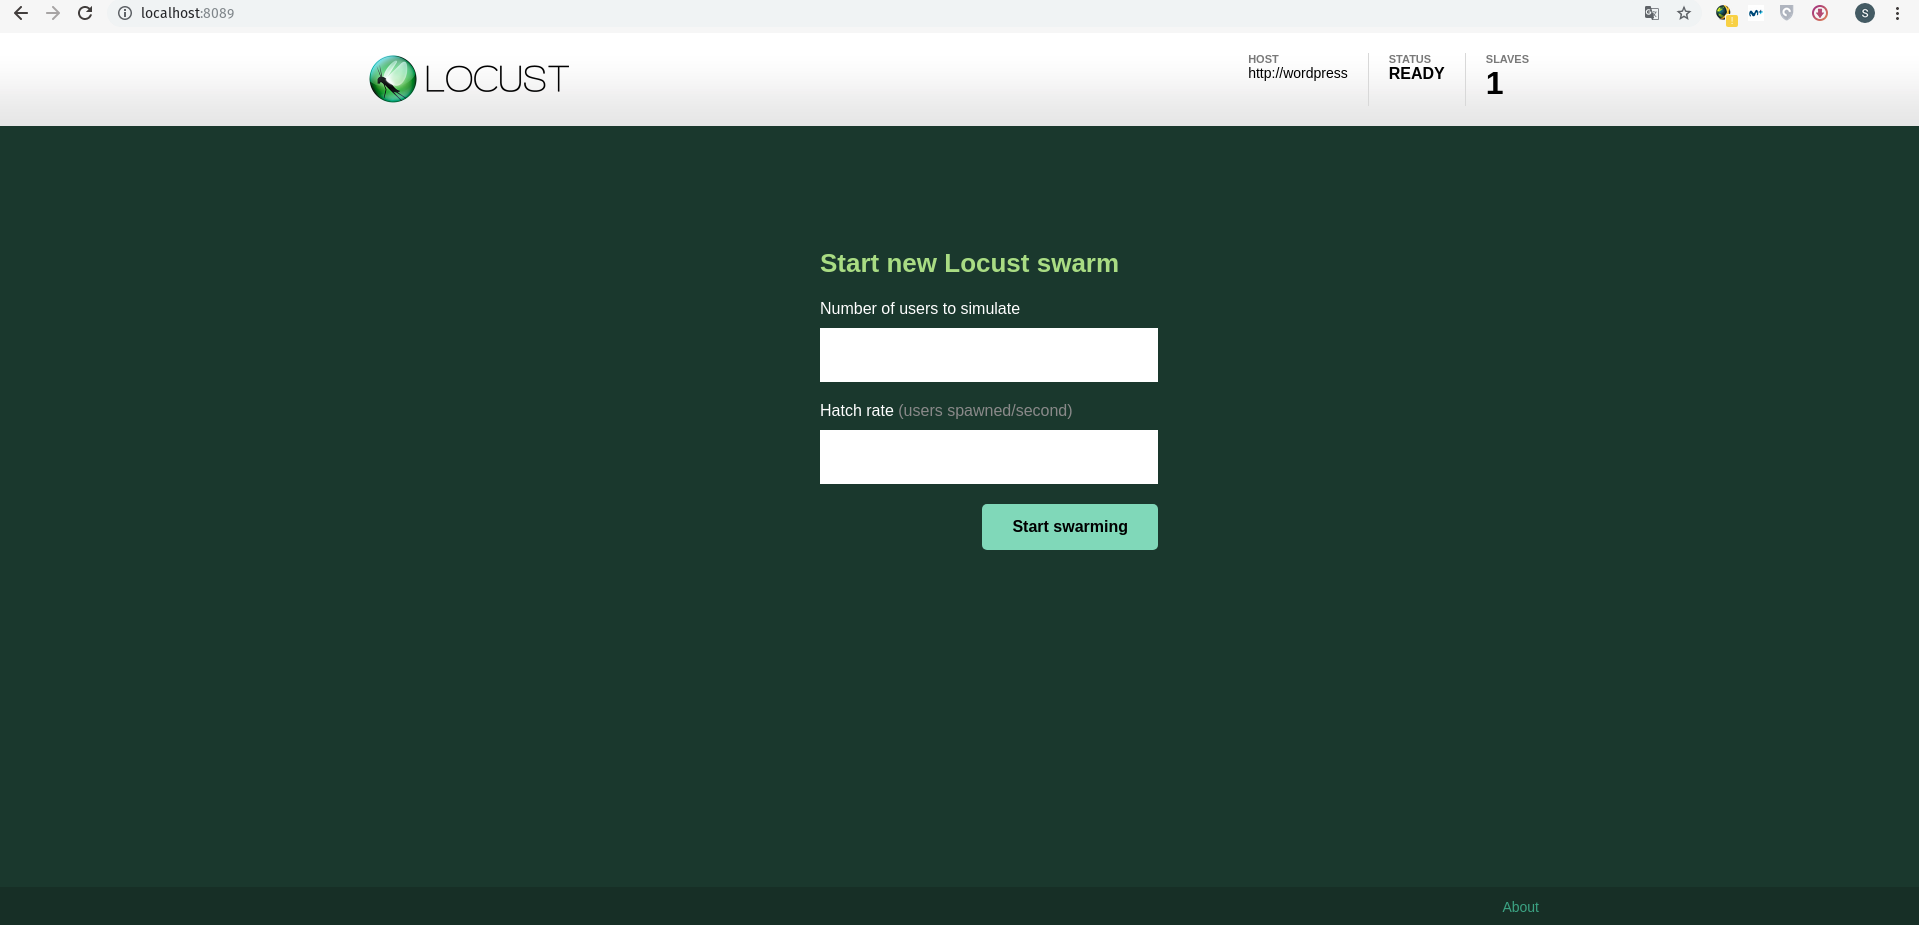
\includegraphics[scale=0.2]{imagenes/carga/locustInterfaz.png}
	\caption{Interfaz Locust} \label{locust_interfaz}
\end{figure}

Si ejecutamos como Number of users con valor 10 y el Hatch rate con valor 1 tenemos que cuando se inicie la prueba de carga con esta configuración, Locust generará 1 nuevo usuario por cada segundo hasta que alcance el número total de usuarios a simular (que en este caso es 10). Cuando alcanza el número de usuarios, la estadística se restablecerá.
\newpage
Esta explicación viene representada de forma gráfica de la siguiente manera:

\begin{figure}[H]
	\centering
	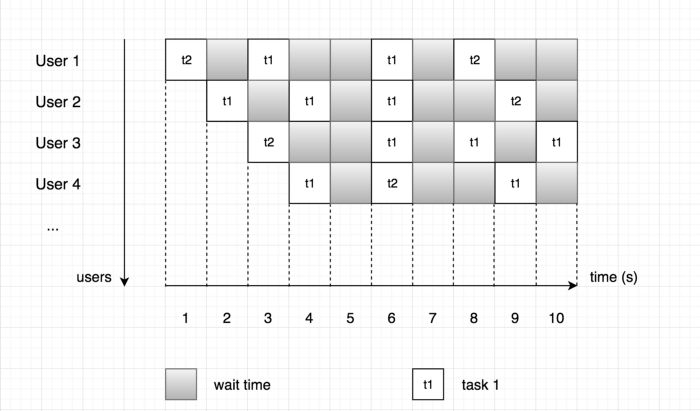
\includegraphics[scale=0.2]{imagenes/carga/explicacion_locust.png}
	\caption{Realización de tareas concurrentes} \label{locust}
\end{figure}

Después de establecer estos valores, se podrá ver el resultado de la prueba en tiempo real:
\begin{figure}[H]
	\centering
	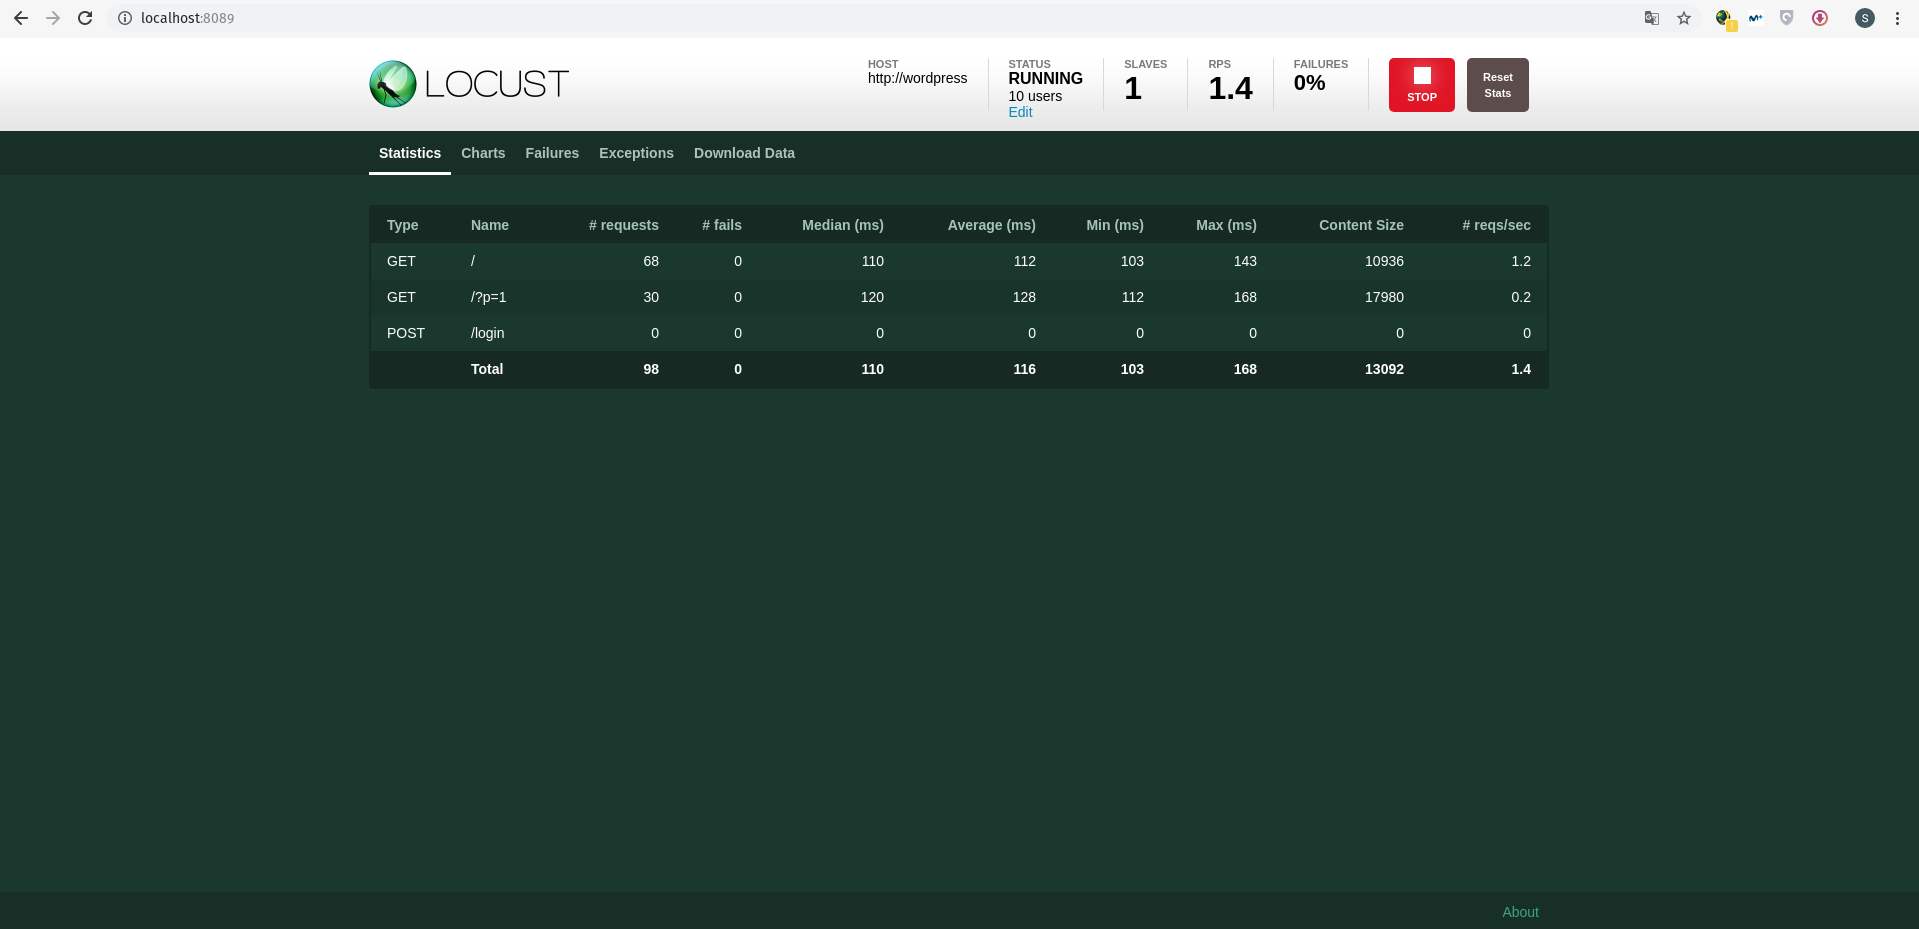
\includegraphics[scale=0.2]{imagenes/carga/pruebalocust.png}
	\caption{Pruebas de tareas concurrentes} \label{locust_prueba}
\end{figure}

Una vez que se ha alcanzado el número deseado de solicitudes, se puede detener la herramienta \textbf{Locust }desde la interfaz web. También permite restablecer las estadísticas o ejecutar una nueva prueba o test.
Además de las estadísticas, puede mirar los \textbf{gráficos} (segunda pestaña) o cualquier \textbf{fallo o excepción que se haya recibido} (tercera, cuarta pestaña), así como \textbf{descargar los resultados de las pruebas como archivos CSV} (la última pestaña).
\newpage
\begin{figure}[H]
	\centering
	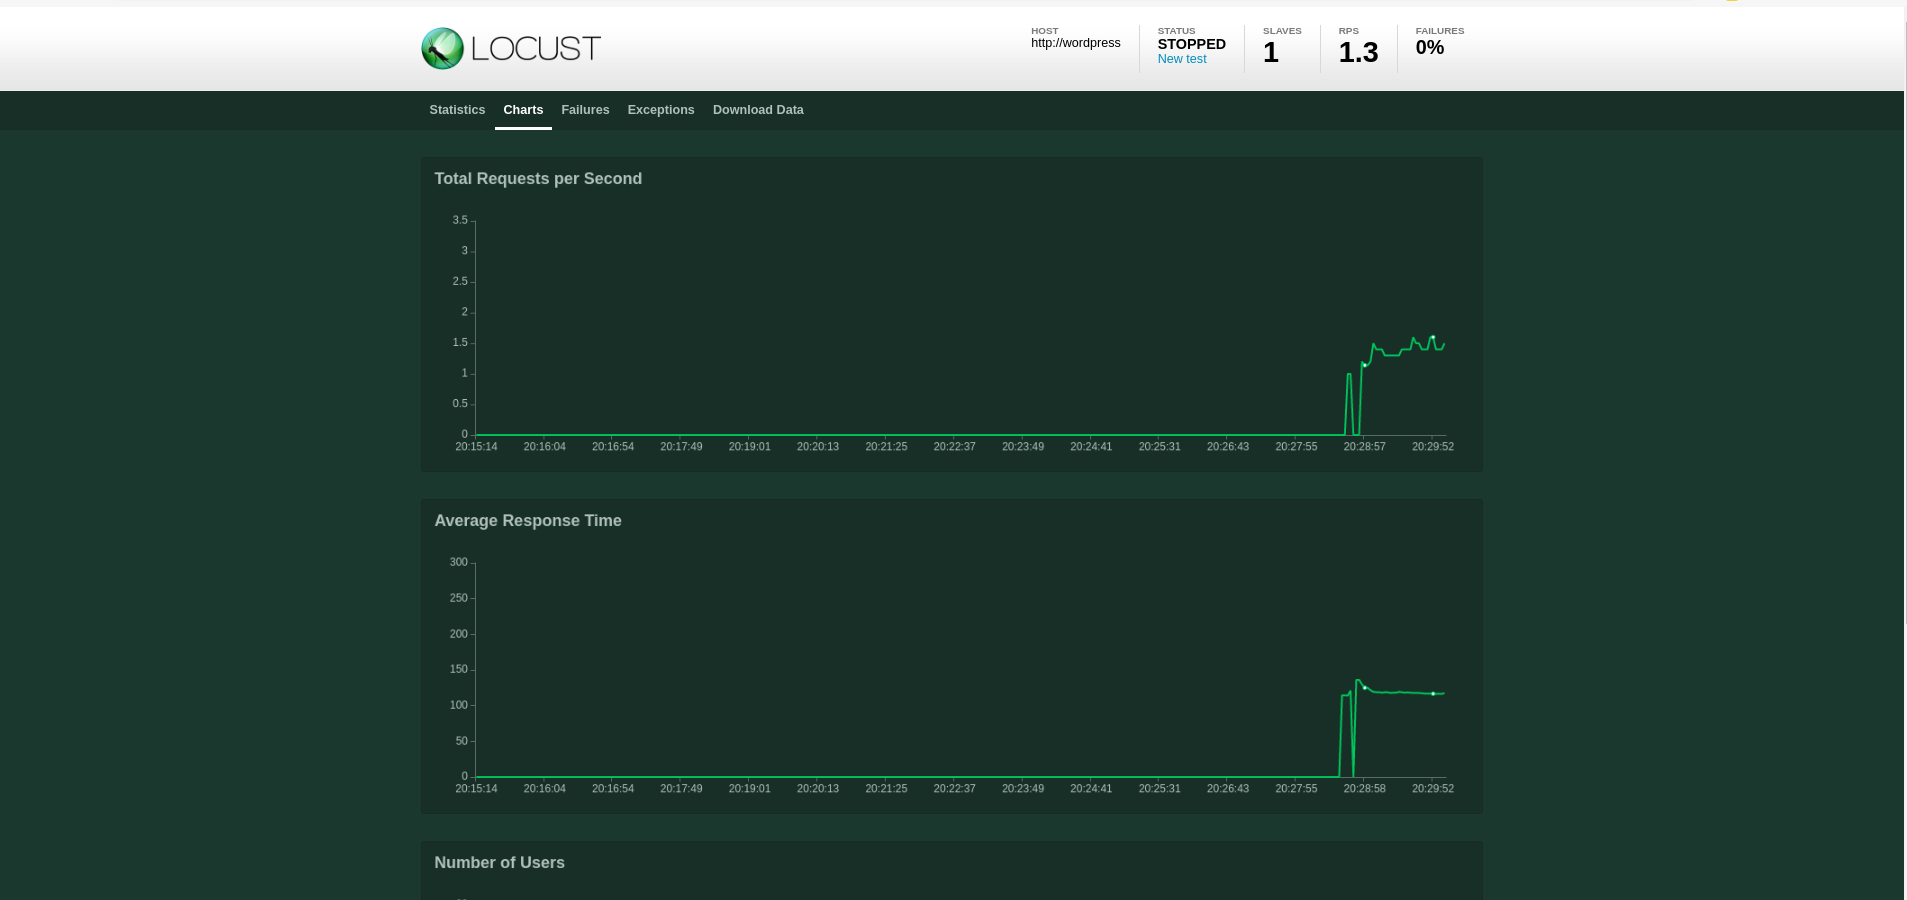
\includegraphics[scale=0.2]{imagenes/carga/charts.png}
	\caption{Gráfico generado en las ejecuciones} \label{locust_chart}
\end{figure}

Básicamente, las\textbf{ solicitudes por segundo}, es decir, el \textbf{rendimiento} indican la cantidad de transacciones por segundo que la aplicación puede realizar.

El \textbf{tiempo de respuesta }es la cantidad de tiempo desde el momento en que un usuario envía una solicitud hasta el momento en que su aplicación indica que la solicitud se ha completado.
 
En el gráfico anterior se puede ver la correlación entre los \textbf{tiempos de respuesta y el rendimiento}. El \textbf{rendimiento} general tiende a disminuir a medida que aumenta el tiempo de respuesta para una transacción promedio. El \textbf{motivo} es que después de enviar la primera solicitud, \textbf{Locust} debe esperar hasta que la solicitud se complete o se procese para enviar la segunda solicitud. 

\section{Pruebas de monitorización en Naemon}
En esta sección vamos a empezar con  la \textbf{puesta en marcha de la herramienta Naemon a través del análisis del sistema realizado}, es decir, el sistema WordPress. Como se señaló en el capítulo \ref{ch:estado}, donde especificabamos la carpeta de configuración de los distintos equipos y servicios a monitorizar, esta es la carpeta \textbf{/etc/naemon/conf.d}, en esta carpeta aplicaremos la configuración correspondiente para analizar el sistema WordPress.
\newpage
Por defecto, Naemon configura la siguiente estructura de archivos y carpetas dentro de la carpeta anterior:
\begin{figure}[H]
	\centering
	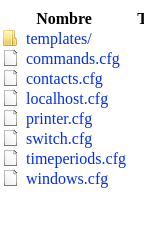
\includegraphics[scale=0.7]{imagenes/wordpress/analisis_naemon/estructura_1.png}
	\caption{Contenido de /etc/naemon/conf.d} \label{conf}
\end{figure}
Dentro de la carpeta \textbf{templates} encontramos el siguiente contenido:
\begin{figure}[H]
	\centering
	
\includegraphics[scale=0.5]{imagenes/wordpress/analisis_naemon/estructura_templates.png}
	\caption{Contenido de /etc/naemon/conf.d/templates} \label{templates}
\end{figure}

Dentro de la carpeta \textbf{templates} podemos encontrar plantillas de ejemplos de hosts y services, donde el contenido de estos lo vamos a aplicar en la creación de nuestros archivos de configuración.
\newpage
El archivo \textbf{localhost.cfg} es una plantilla de ejemplo del analisis de un servidor linux, tomaremos de ejemplo este para realizar las diferentes configuraciones, para poder introducir nuestros nuevos archivos de configuración, debemos modificar la imagen que creamos anteriormente para desplegar Naemon, donde incluiremos las siguientes líneas, donde añadiremos un archivo de incorporación de hosts y de servicios, además de eliminar dicho archivo \textbf{localhost.cfg}:

\begin{lstlisting}[language=bash]
RUN rm -rf /etc/naemon/conf.d/localhost.cfg
ADD definition/wordpresshosts.cfg /etc/naemon/conf.d/wordpresshosts.cfg 
ADD definition/wordpressservices.cfg /etc/naemon/conf.d/wordpressservices.cfg 
\end{lstlisting}

A continuación se muestra el \textbf{contenido} de los dos nuevos archivos:

\begin{figure}[H]
	\centering
	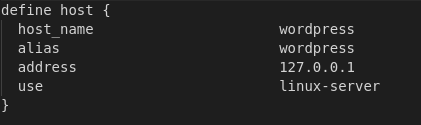
\includegraphics[scale=0.4]{imagenes/wordpress/analisis_naemon/host.png}
	\caption{Contenido del archivo de configuración del host} \label{host}
\end{figure}

\begin{figure}[H]
	\centering
	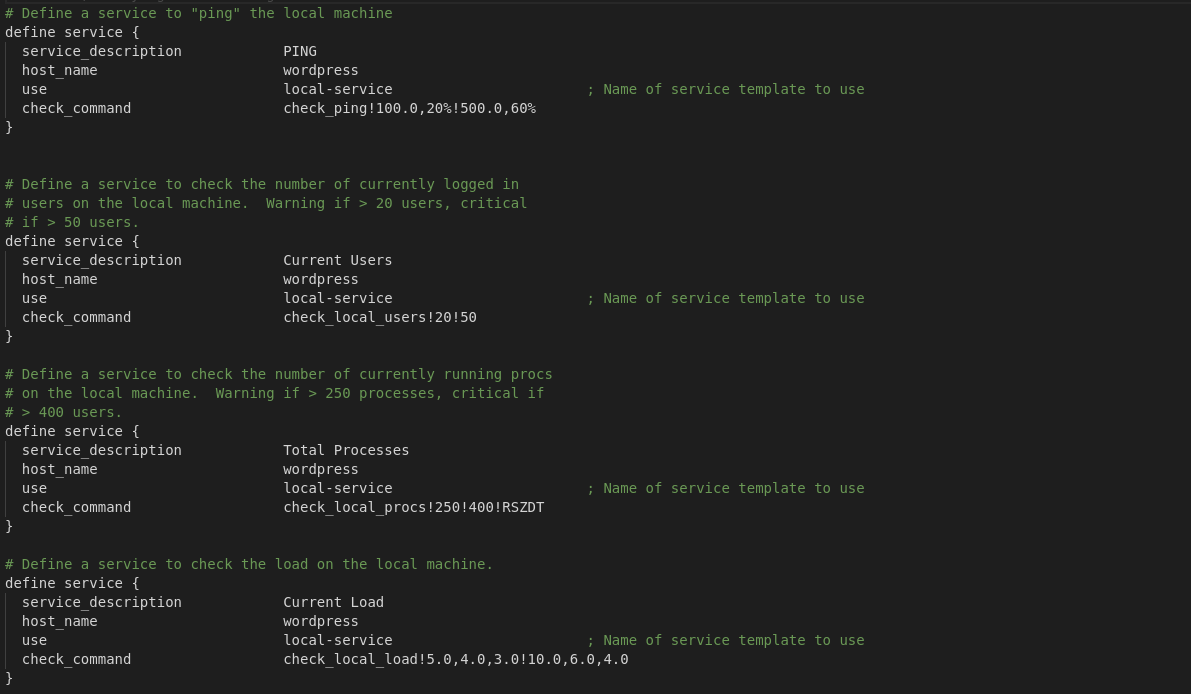
\includegraphics[scale=0.3]{imagenes/wordpress/analisis_naemon/services1.png}
	\caption{Contenido del archivo de configuración del services} \label{services1}
\end{figure}
\newpage
\begin{figure}[H]
	\centering
	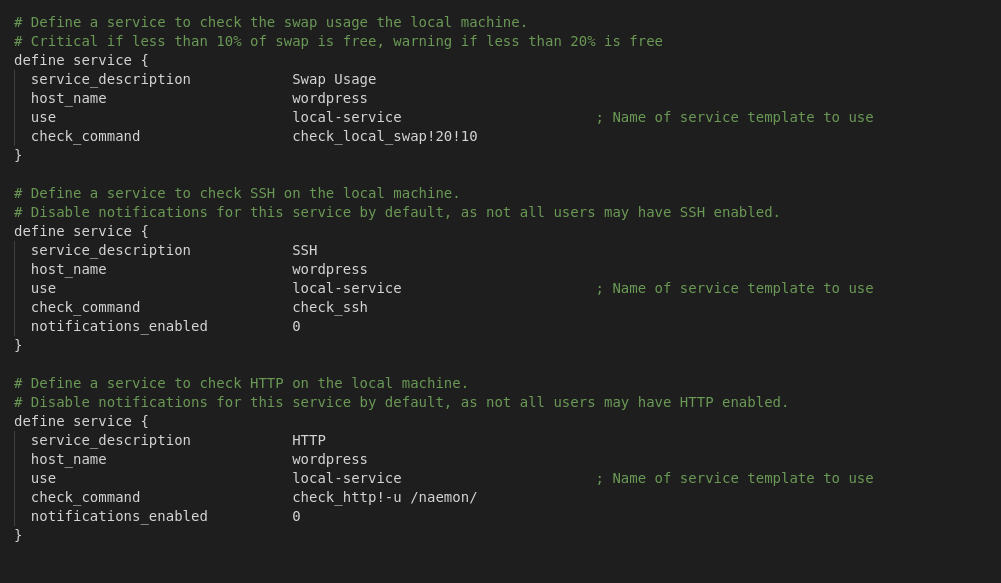
\includegraphics[scale=0.3]{imagenes/wordpress/analisis_naemon/services2.png}
	\caption{Contenido del archivo de configuración del services} \label{services2}
\end{figure}
En los siguientes apartados, se explicará las definiciones que se han realizado.
\subsection{Definición del host}

A través del archivo llamado con el nombre \textbf{wordpresshosts.cfg} se ha realizado la definición del host correspondiente al sistema wordpress, donde a través de:

\begin{itemize}
	\item La etiqueta \textbf{host\_name}, asigna el nombre del host, el cual se ha designado como \textbf{wordpress}.
	\item La etiqueta \textbf{alias},asigna un alias al host, el cual se ha designado como \textbf{wordpress}.
	\item La etiqueta \textbf{address},se encarga de establecer la dirección IP donde se encontrará el host ubicado. Estableceremos \textbf{127.0.0.1 }que será nuestro \textbf{localhost}
	\item La etiqueta \textbf{use}, esta etiqueta se utiliza para usar una plantilla concreta, en este caso usaremos la creada por Naemon, la llamada \textbf{linux-server}, que hablaremos de ella a continuación.
\end{itemize}
\newpage
El host utilizado \textbf{linux-server} se trata de un host creado por Naemon, que no contiene funcionalidad, pero utilizaremos como plantilla para poder trabajar, ya que este se encarga de definir el tiempo por el cual va a estar trabajando el host, además de comprobar en todo momento si está en activo, mediante el plugin \textbf{check-host-alive}. Este host se basa en \textbf{generic-host}, ésta se trata de otra plantilla, a continuación mostramos el contenido de cada plantilla de los host:
 

\begin{lstlisting}[language=bash]

define host {
	name                           generic-host                        ; 
	event_handler_enabled          1                                   ; 
	flap_detection_enabled         1                                   ; 
	notification_period            24x7                                ; 
	notifications_enabled          1                                   ; 
	process_perf_data              1                                   ; 
	register                       1                                   ; 
	retain_nonstatus_information   1                                   ; 
	retain_status_information      1                                   ; 
}


define host {
	name                           linux-server                        ; 
	use                            generic-host                        ; 
	check_command                  check-host-alive                    ; 
	check_interval                 5                                   ; 
	check_period                   24x7                                ; 
	contact_groups                 admins                              ; 
	max_check_attempts             10                                  ; 
	notification_interval          120                                 ; 
	notification_options           d,u,r                               ; 
	notification_period            workhours                           ; 
	register                       1                                   ; 
	retry_interval                 1                                   ; 
}

\end{lstlisting}
\newpage
Las directivas de la definición de los host se explicaron en el capítulo de Estado de Arte \ref{ch:estado}, en este caso el funcionamiento concreto que se ha establecido para el host \textbf{generic-host} es el siguiente:

\begin{itemize}
	\item A través de la directiva \textbf{event\_handler\_enabled} a 1 hemos habilitado el controlador de eventos del host.
	\item A través de la directiva \textbf{flap\_detection\_enabled} a 1 hemos habilitado la detección de flaps del host.
	\item A través de la directiva \textbf{notification\_period} se ha indicado que esté dispuesto 24h a la semana.
	\item A través de la directiva \textbf{notifications\_enabled} a 1 hemos habilitado las notificaciones del host.
	\item A través de la directiva \textbf{process\_perf\_data} a 1 habilita el procesamiento de datos de rendimiento.
	\item A través de la directiva \textbf{register} a 1 hace que se registre el host.
	\item A través de la directiva \textbf{retain\_nonstatus\_information} a 1 habilita la retención de información sin estado.
	\item A través de la directiva \textbf{retain\_status\_information} a 1 habilita la retención de información de estado.
\end{itemize}

El funcionamiento concreto que se ha establecido para el host \textbf{linux-server} es el siguiente:

\begin{itemize}
	\item A través de la directiva \textbf{use} hace que herede la información de generic-host.
	\item A través de la directiva \textbf{check\_command} se intentará hacer un ping al host para ver si está vivo o activado.
	\item A través de la directiva \textbf{check\_interval} se establecerá el valor 5 como unidad de tiempo entre las distintas comprobaciones realizadas.
	\item A través de la directiva \textbf{check\_period} se activará una comprobación de 24h a la semana.
	\item A través de de la directiva \textbf{contact\_groups} se especificará que el grupo al que se notificará es al creado llamado admins.
	\item A través de la directiva \textbf{max\_check\_attempts} con valor 10, indicará que realizará diez veces el intento del comando de verificación del host.
	\newpage
	\item A través de la directiva \textbf{notifications\_enabled} a 1 hemos habilitado las notificaciones del host.
	\item A través de la directiva \textbf{notification\_period} se ha indicado que esté dispuesto en horas laborables.
	\item A través de la directiva \textbf{register} a 1 hace que se registre el host.
	
\end{itemize}

\subsubsection{Host utilizado en la prueba de monitorización del sistema}

En la figura \ref{host} se muestra la configuración del host que se va a utilizar en nuestra prueba, para ello aplicaremos el uso de la plantilla ya creada y explicada \textbf{linux-server}, lo único que tendremos que especificar para la creación de este nuevo host es la \textbf{dirección IP} desde donde se va encontrar el host creado y el nombre del nombre, el cual llamaremos como el sistema utilizado, es decir, \textbf{wordpress}.

Si accedemos a Naemon a través de la GUI de Thruk, podremos ver reflejado la creación de este nuevo host. La información establecida del host vendrá reflejado en la figura \ref{wordpresshost}.
\begin{figure}[H]
	\centering
	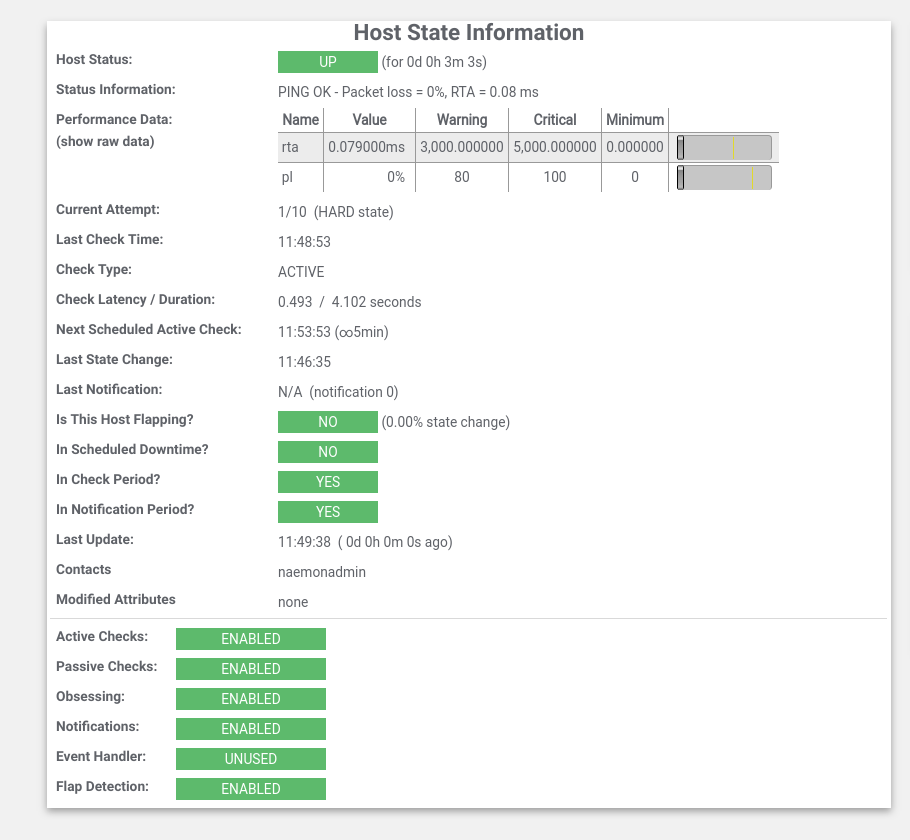
\includegraphics[scale=0.3]{imagenes/wordpress/analisis_naemon/wordpress_host.png}
	\caption{Información del host en Naemon} \label{wordpresshost}
\end{figure}
\newpage
Como podemos observar el host se encuentra activo, ya que su estado es \textbf{UP}, además al indicarle que heredase las directivas de linux-server aparecerán también reflejadas en la información anteriormente mostrada.

En este caso a la hora de ejecutar el \textbf{PING}, servicio que explicaremos en el apartado siguiente, hacia este host, podemos ver que lo realiza de forma correcta, por lo que no se genera pérdida de datos ni paquetes, ya que además en la información mostrada se puede apreciar ese dato. Además mostrará el valor del \textbf{RTA} o lo que es lo mismo \textit{``round trip average"}, que medirá la velocidad de transferencia de los datos, siendo este un valor bastante reducido como se muestra en la figura \ref{wordpresshost}.

\subsection{Definición de los servicios}
A través de este archivo, definiremos los \textbf{servicios} que usaremos en los \textbf{chequeos} o comprobaciones. Se define la métrica o el servicio a monitorizar sobre el que se ejecuta.
Como en el caso del host se ha establecido el uso de la plantilla aportada por Naemon, es decir, se ha utilizado la plantilla \textbf{local-service}.

\begin{lstlisting}[language=bash]

define service {
	name                           generic-service                     ; 
	active_checks_enabled          1                                   ; 
	check_freshness                0                                   ; 
	check_interval                 10                                  ; 
	check_period                   24x7                                ; 
	contact_groups                 admins                              ; 
	event_handler_enabled          1                                   ; 
	flap_detection_enabled         1                                   ; 
	is_volatile                    0                                   ; 
	max_check_attempts             3                                   ; 
	notification_interval          60                                  ; 
	notification_options           w,u,c,r                             ; 
	notification_period            24x7                                ; 
	notifications_enabled          1                                   ; 
	obsess_over_service            1                                   ; 
	passive_checks_enabled         1                                   ; 
	process_perf_data              1                                   ; 
	register                       1                                   ; 
	retain_nonstatus_information   1                                   ; 
	retain_status_information      1                                   ; 
	retry_interval                 2                                   ; 
}


define service {
	name                           local-service                       ; 
	use                            generic-service                     ; 
	check_interval                 5                                   ; 
	max_check_attempts             4                                   ; 
	register                       1                                   ; 
	retry_interval                 1                                   ; 
}

\end{lstlisting}
Las directivas de la definición de los servicios se explicaron en el capítulo de Estado de Arte \ref{ch:estado}, como se ha realizado para la definición del host, a continuación se explicará el funcionamiento a seguir del servicio \textbf{generic-service} y \textbf{local-service}.

Para \textbf{generic-service} las directivas de funcionamiento establecidas son las siguientes:
\begin{itemize}
	
	\item \textbf{is\_volatile}: lo establecemos a 0 para indicar que no será un servicio volátil, es decir, no queremos que se pierda o se elimine la información recogida por el servicio.
	\item \textbf{max\_check\_attempts}:se utiliza para definir la cantidad de veces que Naemon volverá a intentar el comando de verificación de servicio si devuelve cualquier estado que no sea OK. 	Por lo que esto lo realizará una cantidad de tres veces.
	\item \textbf{check\_interval}: se establecerá el valor 10 como unidad de tiempo entre las distintas comprobaciones realizadas.
	\item \textbf{retry\_interval}: se establecerá el valor 2 como unidad de tiempo a esperar antes de programar una nueva verificación del servicio.
	\newpage
	\item \textbf{active\_checks\_enabled}: habilita las comprobaciones activas del servicio.
	\item \textbf{passive\_checks\_enabled}: habilita las comprobaciones pasivas del servicio.
	\item \textbf{check\_period}: se activará una comprobación de 24h a la semana.	
	\item \textbf{obsess\_over\_service|obsess}	: habilita las comprobaciones para el servicio estarán sobrecargadas con el uso del comando ocsp\_command. 
	\item \textbf{check\_freshness}: deshabilita las comprobaciones de actualización ya que esto puede suponer una carga sobre el servicio. 	
	\item \textbf{event\_handler\_enabled}: habilita el controlador de eventos de servicio.
	\item \textbf{flap\_detection\_enabled}: habilita la detección de flaps de servicio.
	\item \textbf{process\_perf\_data}:habilita el procesamiento de datos de rendimiento.
	\item \textbf{retain\_status\_information}: habilitar la retención de información de estado.
	\item \textbf{retain\_nonstatus\_information}: habilitar la retención de información sin estado.
	\item \textbf{notification\_interval}: esperará 60 minutos para volver a notificar a un contacto que este servicio todavía está en un estado no correcto.	

	\item \textbf{notification\_period}: se ha indicado que esté dispuesto 24h a la semana.
	\item \textbf{notification\_options}: se enviarán notificaciones en caso de estado de ADVERTENCIA, DESCONOCIDO, CRÍTICO Y RECUPERACIÓN. 
	\item \textbf{notifications\_enabled}: habilitar notificaciones de servicio. 
	\item \textbf{contact\_groups}: notificará a los grupos administrados, identificados como \textbf{admins}.
	
\end{itemize}
\newpage
Para \textbf{local-service} las directivas de funcionamiento establecidas son las siguientes:
\begin{itemize}	
	\item \textbf{use}: indicará que heredará las directivas de generic-service.
	\item \textbf{max\_check\_attempts}:se utiliza para definir la cantidad de veces que Naemon volverá a intentar el comando de verificación de servicio si devuelve cualquier estado que no sea OK. 	Por lo que esto lo realizará una cantidad de cinco veces.
	\item \textbf{check\_interval}: se establecerá el valor 4 como unidad de tiempo entre las distintas comprobaciones realizadas.
	\item \textbf{retry\_interval}: se establecerá el valor 1 como unidad de tiempo a esperar antes de programar una nueva verificación del servicio.
	\item A través de la directiva \textbf{register} a 1 hace que se registre el servicio.

\end{itemize}
\subsubsection{Servicios utilizados en la prueba de monitorización del sistema}

En las figuras \ref{services1} y \ref{services2} se muestran la configuración de los servicios que se van a utilizar en nuestra prueba, para ello aplicaremos el uso de la plantilla ya creada y explicada \textbf{local-service y generic-service}.

Si accedemos a \textbf{Naemon} a través de la \textbf{GUI de Thruk}, podremos ver reflejada la creación de estos servicios. La información establecida del host con cada servicio vinculado vendrá reflejado en la figura \ref{wordpressservices}.
\begin{figure}[H]
	\centering
	
	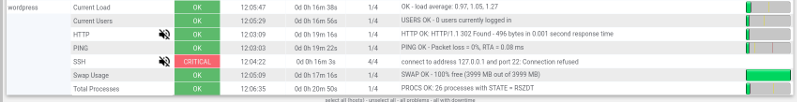
\includegraphics[scale=0.4]{imagenes/wordpress/analisis_naemon/wordpress_services.png}
	\caption{Información del host con cada servicio vinculado en Naemon} \label{wordpressservices}
\end{figure}
A continuación vamos a hablar en detalle de cada servicio definido en el archivo \textbf{wordpressservices.cfg}. 
\newpage
\paragraph{Servicio PING}

A través de la directiva check\_command haremos uso del plugin \textbf{check\_ping}, por el cual hacemos uso de la llamada PING para comprobar las estadísticas de conexión del host.

Para este plugin se establecerá el \textbf{umbral $<$rta$>$,$<$pl$>$} donde \textbf{$<$rta$>$} será el tiempo o la velocidad de transferencia media en "ms" que activará un estado de \textbf{WARNING(advertencia) o CRITICAL(crítico)}, además \textbf{$<$pl$>$} es el porcentaje de pérdida de paquetes para activar un estado de alarma.

El uso de este comando suele ser de la siguiente forma:
\begin{lstlisting}
check_ping -H <host_address> -w <wrta>,<wpl>% -c <crta>,<cpl>%
[-p packets] [-t timeout] [-4|-6]

\end{lstlisting}

La función de check\_command aplicará dicho comando plugin con la siguiente forma de definición:
\begin{lstlisting}
check_ping!100.0,20%!500.0,60%
\end{lstlisting} 

Donde se asume que:
\begin{itemize}
	\item Para el estado \textbf{WARNING}: $<$wrta$>$ es 100.0 y $<$wpl$>$ es 0,20.
	\item Para el estado \textbf{CRITICAL}: $<$crta$>$ es 500.0 y $<$cpl$>$ es 0,60
\end{itemize}

Si este comando se accediera a través de una terminal o línea de comandos de forma expandida, se escribiría de la siguiente forma:

\begin{lstlisting}
/usr/lib/naemon/plugins/check_ping -H 127.0.0.1 -w 100.0,20% -c 500.0,60% -p 5
\end{lstlisting}

Donde se establece el host y el número de paquetes a enviar que si no se asume nada se toma por defecto el valor 5.

Este plugin utiliza el comando \textbf{ping} para que el host especificado busque la pérdida de paquetes según un porcentaje y el promedio de ida y vuelta en milisegundos.
\newpage
Si accedemos a la \textbf{GUI de Thruk} podemos observar el registro de información del rendimiento, obteniéndose los siguientes valores:
 
\begin{lstlisting}
rta=0.087000ms;100.000000;500.000000;0.000000 pl=0%;20;60;0
\end{lstlisting}

Por lo que el estado que obtendremos será \textbf{OK}, ya que no se ha perdido ningún paquete y los valores del \textbf{RTA} son tan pequeños que no se encuentran en el estado de \textbf{WARNING ni CRITICAL}.

\paragraph{Servicio para comprobar usuarios actuales registrados}

A través de la directiva \textbf{check\_command} haremos uso del siguiente plugin \textbf{check\_local\_users}, con este plugin comprobaremos el número de usuarios que se encuentran registrados en el servidor o host y genera un error si el número excede los umbrales especificados.

Para este plugin se establecerá el \textbf{umbral para warning y critical}.

El uso de este comando suele ser de la siguiente forma:
\begin{lstlisting}
check_local_users -w <users> -c <users>
\end{lstlisting}

La función de check\_command aplicará dicho comando plugin con la siguiente forma de definición:
\begin{lstlisting}
check_local_users!20!50
\end{lstlisting} 

Donde se asume que:
\begin{itemize}
	\item Para el estado \textbf{WARNING}: se ha establecido un límite de 20 usuarios.
	\item Para el estado \textbf{CRITICAL}: se ha establecido un límite de 50 usuarios.
\end{itemize}

Si este comando se accediera a través de una terminal o línea de comandos de forma expandida, se escribiría de la siguiente forma:

\begin{lstlisting}
/usr/lib/naemon/plugins/check_users -w 20 -c 50
\end{lstlisting}
\newpage
Si accedemos a la \textbf{GUI de Thruk} podemos observar el registro de información del rendimiento, obteniéndose los siguientes valores:

\begin{lstlisting}
USERS OK - 0 users currently logged in

users=0;20;50;0
\end{lstlisting}

Por lo que el estado que obtendremos será \textbf{OK}, ya que no se ha excedido los valores asignados en cuanto a usuarios conectados.
\paragraph{Servicio para comprobar total de procesos ejecutados}

A través de la directiva \textbf{check\_command} haremos uso del siguiente plugin \textbf{check\_local\_procs}, con este plugin comprobaremos todos los procesos y generaremos estados de ADVERTENCIA o CRÍTICOS si la métrica especificada está fuera de los rangos de umbral requeridos. El valor predeterminado de la métrica es el número de procesos. Los filtros de búsqueda se pueden aplicar para limitar los procesos a verificar.

El uso de este comando suele ser de la siguiente forma:
\begin{lstlisting}
check_local_procs -w <range> -c <range> [-m metric] [-s state] [-p ppid]
[-u user] [-r rss] [-z vsz] [-P %cpu] [-a argument-array]
[-C command] [-k] [-t timeout] [-v]
\end{lstlisting}

La función de \textbf{check\_command} aplicará dicho comando plugin con la siguiente forma de definición:
\begin{lstlisting}
check_local_procs!250!400!RSZDT
\end{lstlisting} 

Donde se asume que:
\begin{itemize}
	\item Para el estado \textbf{WARNING}: se ha establecido un límite de 250 procesos.
	\item Para el estado \textbf{CRITICAL}: se ha establecido un límite de 400 procesos.
	\item Se ha establecido el estado \textbf{RSZDT}, el cual significa lo siguiente: \textbf{R:ejecutable,S:esperando de forma dormida,Z:proceso zombie que termina pero no se repite por su padre, D: ininterrumpible, T:parado por una señal de control}.
\end{itemize}
\newpage
Si este comando se accediera a través de una terminal o línea de comandos de forma expandida, se escribiría de la siguiente forma:

\begin{lstlisting}
/usr/lib/naemon/plugins/check_procs -w 250 -c 400 -s RSZDT
\end{lstlisting}

Si accedemos a la \textbf{GUI de Thruk} podemos observar el registro de información del rendimiento, obteniéndose los siguientes valores:

\begin{lstlisting}
PROCS OK: 26 processes with STATE = RSZDT

procs=26;250;400;0;
\end{lstlisting}

Por lo que el estado que obtendremos será \textbf{OK}, ya que no se ha excedido los valores asignados en cuanto a procesos creados.
\paragraph{Servicio para comprobar la carga actual}

A través de la directiva check\_command haremos uso del plugin \textbf{check\_local\_load}, con este plugin comprobaremos el promedio de carga actual del sistema.

El uso de este comando suele ser de la siguiente forma:
\begin{lstlisting}
check_local_load [-r] -w WLOAD1,WLOAD5,WLOAD15 -c CLOAD1,CLOAD5,CLOAD15 [-n NUMBER_OF_PROCS]
\end{lstlisting}

\begin{itemize}
	\item Donde\textbf{ -r }se encarga de dividir el porcentaje de carga por el número de CPUs, pero esto solo cuando sea posible.
	\item Notificará con el estado de \textbf{ADVERTENCIA} si el promedio de carga excede el valor asignado en WLOADn
	\item Notificará con el estado de \textbf{CRÍTICO} si el promedio de carga excede el valor asignado en CLOADn
\end{itemize}


La función de \textbf{check\_command} aplicará dicho comando plugin con la siguiente forma de definición:
\begin{lstlisting}	
check_local_load!5.0,4.0,3.0!10.0,6.0,4.0
\end{lstlisting} 
\newpage
Donde se asume que:
\begin{itemize}
	\item Para el estado \textbf{WARNING}: se ha establecido las cargas de 5.0, 4.0 y 3.0
	\item Para el estado \textbf{CRITICAL}: se ha establecido las cargas de 10.0, 6.0 y 4.0	
\end{itemize}

Si este comando se accediera a través de una terminal o línea de comandos de forma expandida, se escribiría de la siguiente forma:

\begin{lstlisting}
/usr/lib/naemon/plugins/check_load -w 5.0,4.0,3.0 -c 10.0,6.0,4.0
\end{lstlisting}

Si accedemos a la \textbf{GUI de Thruk} podemos observar el registro de información del rendimiento, obteniéndose los siguientes valores:

\begin{lstlisting}
OK - load average: 0.35, 0.64, 0.68

load1=0.350;5.000;10.000;0; load5=0.640;4.000;6.000;0; load15=0.680;3.000;4.000;0;
\end{lstlisting}

Por lo que el estado que obtendremos será \textbf{OK}, ya que no se ha excedido los valores asignados en cuanto a carga ejecutada.
\paragraph{Servicio para comprobar el uso de intercambio}

A través de la directiva check\_command haremos uso del plugin \textbf{check\_local\_swap}, con este plugin comprobaremos el espacio de intercambio en la máquina local.

El uso de este comando suele ser de la siguiente forma:
\begin{lstlisting}
check_swap [-av] -w <percent_free>% -c <percent_free>%
-w <bytes_free> -c <bytes_free> [-n <state>]
\end{lstlisting}

\begin{itemize}
	\item Notificará con el estado de \textbf{ADVERTENCIA} si hay menos del porcentaje de espacio de intercambio libre o si hay menos bytes de espacio de intercambio libres.
	\item Notificará con el estado de \textbf{CRÍTICO}  si hay menos del porcentaje de espacio de intercambio libre o si hay menos bytes de espacio de intercambio libres.
\end{itemize}


La función de \textbf{check\_command} aplicará dicho comando plugin con la siguiente forma de definición:
\begin{lstlisting}	
check_local_swap!20!10

\end{lstlisting} 

Donde se asume que:
\begin{itemize}
	\item Para el estado \textbf{WARNING}: se ha establecido a 20 el límite
	\item Para el estado \textbf{CRITICAL}: se ha establecido a 10 el límite
\end{itemize}

Si este comando se accediera a través de una terminal o línea de comandos de forma expandida, se escribiría de la siguiente forma:

\begin{lstlisting}
/usr/lib/naemon/plugins/check_swap -w 20 -c 10
\end{lstlisting}

Si accedemos a la \textbf{GUI de Thruk} podemos observar el registro de información del rendimiento, obteniéndose los siguientes valores:

\begin{lstlisting}
SWAP OK - 100% free (3999 MB out of 3999 MB)

swap=3999MB;0;0;0;3999

\end{lstlisting}

Por lo que el estado que obtendremos será \textbf{OK}, ya que no se ha excedido los valores asignados, esto es debido a que nos encontramos en una máquina local sin tener a cargo una máquina Windows o Linux activada en el host.

\paragraph{Servicio para comprobar el protocolo SSH}

A través de la directiva check\_command haremos uso del plugin \textbf{check\_SSH}, con este plugin comprobaremos \textbf{el protocolo SSH}. Intentará conectarse a un servidor SSH en el servidor y puerto especificados

El uso de este comando suele ser de la siguiente forma:
\begin{lstlisting}
check_ssh  [-4|-6] [-t <timeout>] [-r <remote version>] [-p <port>] <host>
\end{lstlisting}
\newpage
\begin{itemize}
	\item Donde\textbf{ -t } define los segundos antes del tiempo de espera de la conexión por defecto es 10.
	\item Donde\textbf{ -r } alerta si la cadena no coincide con la versión esperada del servidor.
	\item Donde\textbf{ -p } define el puerto a especificar.
	\item Se debe establecer el host por el cual se comprobará la conexión SSH.
\end{itemize}

La función de \textbf{check\_command} aplicará dicho comando plugin con la siguiente forma de definición:
\begin{lstlisting}	
check_ssh
\end{lstlisting} 

Si este comando se accediera a través de una terminal o línea de comandos de forma expandida, se escribiría de la siguiente forma:

\begin{lstlisting}
/usr/lib/naemon/plugins/check_ssh  127.0.0.1
\end{lstlisting}

Si accedemos a la \textbf{GUI de Thruk} podemos observar el registro de información del rendimiento, obteniéndose los siguientes valores:

\begin{lstlisting}
connect to address 127.0.0.1 and port 22: Connection refused
\end{lstlisting}

Esto es debido a que no se dió acceso al puerto 22 a la hora de realizar la creación del \textbf{Dockerfile}.
Esto queda arreglado haciendo una llamada a \textbf{EXPOSE 22} en el archivo \textbf{Dockerfile}.
\newpage
Y además añadiendo un nuevo servicio en \textbf{docker-compose.yml} llamado como el propio protocolo \textbf{ssh}. Esto quedará reflejado de la siguiente forma en dicho archivo:
\begin{lstlisting}
	ssh:
	image: "jdeathe/centos-ssh:2.2.1"
	volumes:
	- "wp_html:/var/www/html"
	- "wp_ssh_keys:/etc/ssh"
	ports:
	- "80:22"
	environment:
	SSH_USER: "wordpress"
	SSH_USER_ID: "65534:65534"
	SSH_USER_HOME: "/var/www"
	SSH_USER_PASSWORD_HASHED: "true"
	SSH_USER_PASSWORD: "wordpress"
	SSH_AUTHORIZED_KEYS: "ssh-rsa AAAAB3NzaC1yc2EAAAADAQABAAABAQC9wfq9fZfn9JicyTq//
	peCAd9gQ7mi4vCIoBzx0zGXmSWsY+4TijbDK2Xb9ZuQw8tyCg9rjZ24W2mvfM6+tpC7nVZRvvsSOji641hN9FamBt34+
	oTeOMXyE1WH5dGDdwLHYYXAo/R/
	yNBlxzT1QaqRjA9PJgcrrV2LsnT/6rbrX1x3mOG0M1KytOTHiHhUlNfRCnGFR
	6Velkx8RNj9z8zI9kqaJTICew1Ss1WFDo+02Ij26Xp4JdK4qCCRGSyv6QTbNekN7
	icp25dYK1XsxTiT+N7CYvgOEEeb/lRRzYX9c0JWbaqhiASLo1cYwkWCONqewjID4OQkYjN9JrqdOnb/"
	restart: "always"
\end{lstlisting}
Con esto tendríamos la conexión SSH asegurada, recibiendo el estado \textbf{OK} en la GUI de Naemon. 
\paragraph{Servicio para comprobar el protocolo HTTP}

A través de la directiva check\_command haremos uso del plugin \textbf{check\_http}, con este plugin comprobaremos el servicio HTTP en el host especificado. Se puede probar
servidores normales (\textbf{http}) y seguros (\textbf{https}).
El uso de este comando suele ser de la siguiente forma:
\begin{lstlisting}
check_http -H <vhost> | -I <IP-address> [-u <uri>] [-p <port>]
[-J <client certificate file>] [-K <private key>]
[-w <warn time>] [-c <critical time>] [-t <timeout>] [-L] [-E] [-a auth]
[-b proxy_auth] [-f <ok|warning|critcal|follow|sticky|stickyport>]
[-e <expect>] [-d string] [-s string] [-l] [-r <regex> | -R <case-insensitive regex>]
[-P string] [-m <min_pg_size>:<max_pg_size>] [-4|-6] [-N] [-M <age>]
[-A string] [-k string] [-S <version>] [--sni] [-C <warn_age>[,<crit_age>]]
[-T <content-type>] [-j method]
\end{lstlisting}
\newpage
La función de \textbf{check\_command} aplicará dicho comando plugin con la siguiente forma de definición:
\begin{lstlisting}	
check_http!-u /naemon/
\end{lstlisting} 

Donde se asume que:
\begin{itemize}
	\item La ruta asignada lo realizará a través de -u asignando la ruta /naemon/
\end{itemize}

Si este comando se accediera a través de una terminal o línea de comandos de forma expandida, se escribiría de la siguiente forma:

\begin{lstlisting}
/usr/lib/naemon/plugins/check_http -I 127.0.0.1 -u /naemon/
\end{lstlisting}

Si accedemos a la \textbf{GUI de Thruk} podemos observar el registro de información del rendimiento, obteniéndose los siguientes valores:

\begin{lstlisting}
HTTP OK: HTTP/1.1 302 Found - 502 bytes in 0.001 second response time

time=0.000893s;;;0.000000;10.000000 size=502B;;;0

\end{lstlisting}

Por lo que el estado que obtendremos será \textbf{OK}, especificando que se ha encontrado el protocolo y el tiempo de respuesta es considerable para su acceso, es decir, realiza una petición GET o POST a dicha ruta asignada.

\section{Puesta en práctica: creación de complemento o plugin}

A continuación para empezar a realizar pruebas crearemos un plugin capaz de comprobar si existe una página concreta, esto es en el caso de que el archivo \textbf{wp-config.php} no se detecte, ya que si no se realiza esta comprobación puede ser que tengamos cuando se realiza el servicio HTTP un OK, cuando este no es el verdadero resultado. Así además se comprueba que la base de datos funciona correctamente. Para comprobar que accede de forma correcta a la base de datos y recoge de forma correcta la información haremos uso del plugin \textbf{check\_http}, aunque realizaremos una modificación, por lo que crearemos un nuevo comando, llamado \textbf{check\_wp\_dominio} y le especificaremos que acceda a la ruta \textbf{/2019/08/16/hola-mundo/}, esta se trata de un artículo concreto de nuestro sistema WordPress.
\newpage
Después para poder hacer uso y mostrar el resultado, definiremos el servicio, donde sólo llamaremos al comando creado heredando como en los anteriores servicios el servicio \textbf{local-service}.

\begin{lstlisting}[language=bash]
define command{
	command_name    check_wp_dominio
	command_line    $USER1$/check_http -H $HOSTADDRESS$ -u /2019/08/16/hola-mundo/
}
define service {
	service_description            WordPress Hola Mundo
	host_name                      wordpress
	use                            local-service                       
	check_command                  check_wp_dominio
}
\end{lstlisting}
En la figura \ref{check_hola_mundo} se muestra el resultado obtenido por el servicio ejecutado anteriormente definido.
\begin{figure}[H]
	\centering
	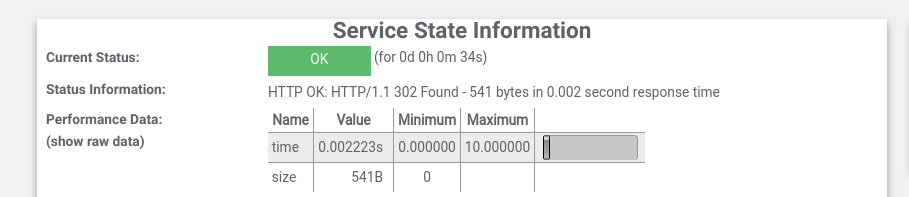
\includegraphics[scale=0.3]{imagenes/wordpress/analisis_naemon/check_hola_mundo.png}
	\caption{Información del estado del plugin de comprobación del puerto 80 sobre la página del artículo Hola, mundo de WordPress} \label{check_hola_mundo}
\end{figure}

Ahora para dar funcionamiento a nuestro sistema y además aplicar la creación de un nuevo plugin o complemento, crearemos uno por el cual compruebe que la ruta indicada por nuestro servicio no se encuentre infectada, es decir, al encontrarnos ante un sistema CMS como WordPress estamos expuestos a gran cantidad de vulnerabilidades externas, por lo que nos apoyaremos de Naemon para monitorizar este estado, para ello crearemos el plugin con nombre \textbf{check\_hackedfiles}.
\newpage
El contenido de este plugin es el siguiente:

\begin{lstlisting}

#!/bin/bash
#

# Config regular expression
REG_EXPR[1]="[0-9a-zA-Z][0-9a-zA-Z][0-9a-zA-Z][0-9a-zA-Z][0-9a-zA-Z][0-9a-zA-Z][0-9a-zA-Z][0-9a-zA-Z][0-9a-zA-Z][0-9a-zA-Z][0-9a-zA-Z][0-9a-zA-Z][0-9a-zA-Z][0-9a-zA-Z][0-9a-zA-Z][0-9a-zA-Z][0-9a-zA-Z][0-9a-zA-Z][0-9a-zA-Z][0-9a-zA-Z]['\"]\.$"
REG_EXPR[2]="[\]x[0-9a-zA-Z][0-9a-zA-Z][\]x[0-9a-zA-Z][0-9a-zA-Z][\]x[0-9a-zA-Z][0-9a-zA-Z][\]x[0-9a-zA-Z][0-9a-zA-Z]"
REG_EXPR[3]="[\]x[0-9a-zA-Z][0-9a-zA-Z][0-9a-zA-Z][\]x[0-9a-zA-Z][0-9a-zA-Z][0-9a-zA-Z]"
REG_EXPR[4]="[\]x[0-9a-zA-Z][0-9a-zA-Z][0-9a-zA-Z][0-9a-zA-Z]"
REG_EXPR[5]="_[0O][0O][0O][0O][0O]"

# EO Config regular expression

# Collection of regular expressions
REG_EXPR=$(printf '%s|' "${REG_EXPR[@]}" | sed 's/|$//')

STATE_OK=0
STATE_WARNING=1
STATE_CRITICAL=2
STATE_UNKNOWN=3

USAGE="Uso: `basename $0` [-h] [-d DIR] [-b NUM] [-l LOG] [-s w/c] [-x FILE]\n
-d [DIR] Directory to check.\n
-b [NUM] Days back.\n
-l [FILE] Log file.\n
-s [w]arning or [c]ritical: Select state when hacked files are present. Default: w\n
-x [FILE] Exclude. List of files to skip check.\n
-e [EXTENSIONS] Exclude file extensions. e.g. \"*.jpg|*.png\"\n
Please use full paths!
"

if [ "$1" == "-h" ] || [ "$1" == "" ] ; then
echo -e $USAGE
exit $STATE_UNKNOWN
fi

while getopts d:b:l:s:x:e: option
do
case "${option}"
in
d) CHECK_DIR=${OPTARG};;
b) DAYS_BACK=${OPTARG};;
l) LOG_FILE=${OPTARG};;
s) RETURN_STATE=${OPTARG};;
x) EXCLUDE_FILES=${OPTARG};;
e) EXCLUDE_FILE_EXTENSIONS=${OPTARG};;
esac
done

### Exit State
if [ -z $RETURN_STATE ]; then
STATE=$STATE_WARNING
else
if [ $RETURN_STATE == "w" ]; then
STATE=$STATE_WARNING
elif [ $RETURN_STATE == "c" ]; then
STATE=$STATE_CRITICAL
else
echo "Bad value for -s!"
echo -e $USAGE
exit $STATE_UNKNOWN
fi
fi
### EO Exit State

### Excludes
if [ -z $EXCLUDE_FILES ]; then
EXCLUDE_PART=""
else
if [ -s "$EXCLUDE_FILES" ]; then 
EXCLUDE_PART=$(printf "! -samefile %s " $(cat $EXCLUDE_FILES))
else
EXCLUDE_PART=""
fi
fi
### EO Excludes

### Exclude file extensions
if [ -z $EXCLUDE_FILE_EXTENSIONS ]; then
EXCLUDE_EXTENSIONS_PART=""
else
EXCLUDE_EXTENSIONS_PART=$(printf "! -name %s " $(echo $EXCLUDE_FILE_EXTENSIONS | sed 's/|/ /g'))
fi
### EO Exclude file extensions

DATE=$(date)

CHECK=$(find $CHECK_DIR -type f \( -name "*" $EXCLUDE_EXTENSIONS_PART $EXCLUDE_PART \) -ctime -$DAYS_BACK -exec grep -lrE "$REG_EXPR" {} \;)

echo "----" >> $LOG_FILE
echo $DATE >> $LOG_FILE

printf '%s\n' "${CHECK[@]}" >> $LOG_FILE


if [ -z "$CHECK" ]; then
echo "OK - There are no infected files for the last $DAYS_BACK days."
exit $STATE_OK
else
echo "There may be infected files from the last $DAYS_BACK days."
exit $STATE
fi

\end{lstlisting}
\newpage
Su \textbf{funcionamiento} es el siguiente:

\begin{itemize}
	\item Dependiendo el valor o la opción a comprobar que se le pase que se le pase, ya sea un directorio, un archivo log, un archivo excluido o un archivo de extensión, parseará con \textbf{getopts} esa opción y la guardará en su correspondiente opción.
	\item Si se ha encontrado con un algún estado \textbf{WARNING O CRITICAL} se encargará de devolver dicho estado.
	\item Empieza la comprobación de cada elementos comprobando que se encuentra dentro del sistema.
	\item En el caso de encontrarse y además contener expresiones regulares que no se encuentran acorde al contenido que deben tener, esta lanzará la opción de que se encuentran infectados y lanzará un \textbf{WARNING o CRITICAL}.
\end{itemize}

Para poder poner este plugin en marcha, es necesario crear el comando correspondiente y su servicio.

\begin{lstlisting}

define command{
	command_name    check_hackedfiles
	command_line    $USER1$/check_hackedfiles $ARG1$
}

define service{
	use                     generic-service,service-pnp    
	host_name               wordpress
	service_description     Hackedfiles
	check_command           check_hackedfiles! /
}

\end{lstlisting}

Este contenido lo ingresaremos en \textbf{wordpresshosts.cfg} y \textbf{wordpressservices.cfg} anteriormente creados y además debemos crear dentro de nuestro \textbf{Dockerfile} la siguiente línea para poder añadir a la carpeta de plugin nuestro archivo nuevo, y le daremos permiso de ejecución:

\begin{lstlisting}
ADD plugins/check_hackedfiles /usr/lib/naemon/plugins/check_hackedfiles
RUN sync && chmod 755 /usr/lib/naemon/plugins/check_hackedfiles
\end{lstlisting}
\newpage
Si lanzamos nuestra ejecución y accedemos a nuestro servicio creado en \textbf{Thruk} podemos visualizar lo reflejado en la figura \ref{check_hackfiles}.

\begin{figure}[H]
	\centering
	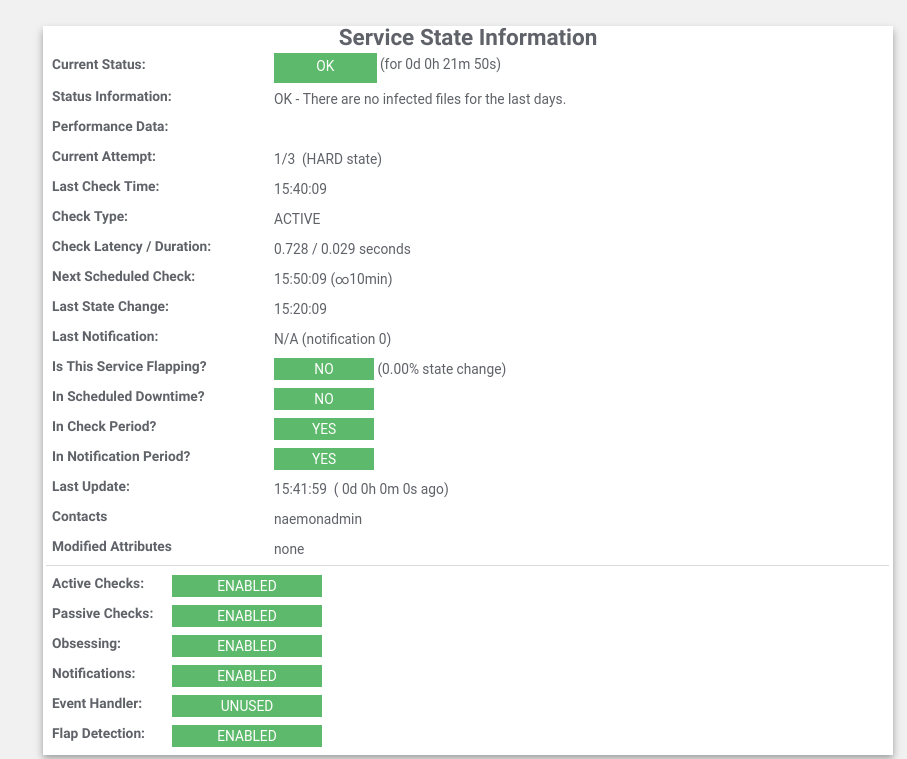
\includegraphics[scale=0.3]{imagenes/wordpress/analisis_naemon/check_hackfiles.png}
	\caption{Información del estado del plugin de comprobación de archivos} \label{check_hackfiles}
\end{figure}

En el capítulo siguiente pasamos a realizar el \textbf{modelado de cargas} de todos los servicios creados en \textbf{Naemon}, es decir, representaremos la carga de trabajo mediante el análisis de prestaciones y crear con esto un modelo.
\newpage